\documentclass[12pt,letterpaper]{article}
\usepackage{lipsum}
\usepackage{amsmath}
\usepackage{graphicx}
\graphicspath{ {} }
\usepackage{authblk}
\usepackage[top=0.8in, bottom= 0.8in, left= 0.8in, right= 0.8in]{geometry}
\usepackage{fancyhdr}

\pagestyle{fancy}
\begin{document}

%title and author details
\title{Laboratory I, Problem 7: Acceleration of a Ball with an Initial Velocity [Revised]}
\author[]{Cole Nielsen}
\date{} %remove date
\affil[]{Physic 1301W TA: Yao Meng}
\pdfpagewidth 8.5in
\pdfpageheight 11in
%
%
\maketitle
%
\abstract{The dependency of an object's acceleration on its initial velocity was tested. A ball was thrown straight down multiple times with different initial velocities. The acceleration for each trial was determined using a camera and motion analysis software. The independence of acceleration from initial velocity was confirmed through fitting and analysis of the aquired data. }

\section{Introduction}
In order to determine the air quality in the city, an apparatus was designed to test air quality. In principle it is a device that is launched straight down off a tall building to quickly force air through device so it can be tested. The apparatus contains sensitive components that are easily damaged by excessive acceleration, and there is uncertainty of whether acceleration is dependent on its initial velocity \(v_i\). To ensure the device isn't damaged by excessive acceleration due to it's initial velocity \(v_i\), the relationship between an apparatus' initial velocity and its acceleration must be understood. This experiment therefore seeks to determine if there is a relationship between the initial velocity and acceleration of an object. It will do so by determining the acceleration of a tennis ball of fixed mass \(m_{ball}\) projected downward at several different initial velocities.
\section{Prediction}
It is predicted that the acceleration of the apparatus will be independent of its initial velocity, assuming that this scenario neglects air resistance. The only acceleration that should be expected as it is a free falling object is acceleration due to gravity near Earth's surface, or \(g\) at \(-9.81 \frac{m}{s^2}\). Mathematically \(v_i\) doesn't affect acceleration:
\begin{equation}
a(t) = \frac{dv(t)}{dt} = \frac{d}{dt}(at+v_i) = a
\end{equation}
\pagebreak
\section{Procedure}
A tennis ball was thrown downward three seperate times, with only the initial velocity \(v_i\) changing for each trial. The same tennis ball was used for each trial, so the size and mass remains constant. The free fall trajectory of the tennis ball in each trial was recorded with a camera. Motionlab video analysis software was then used to aquire data points (y-position and time) across the trajectory of the ball for each trial. The software does this by calculating the change in position of the ball in the camera's frame based upon a reference length of an object in the frame and the change of time (\(\frac{1}{30}\) second) between frames. The equation for velocity as a function of time \(v(t)\) was found by fitting a line to the velocity-vs-time scatter plots generated by Motionlab. Those results were then used to fit position as a function of time \(y(t)\) of parabolic curves using an initial point on each scatter plot and the integral of the previously found \(v(t)\) function for each trial. Those were then adjusted to find the equations for upper and lower tolerances of each trial. Finally the acceleration acting on the ball for each trial was found by taking the second-derivative for every position as a function of time equation of each trial.
\section{Data}

For each trial, the original graphs from Motionlab will be included followed by improved plots generated using Gnuplot with better fitted lines/curves and tolerance lines/curves. After the graphs, the equations shown in the graphs will be listed.
\newline

\textbf{Trial 1}
\newline\newline
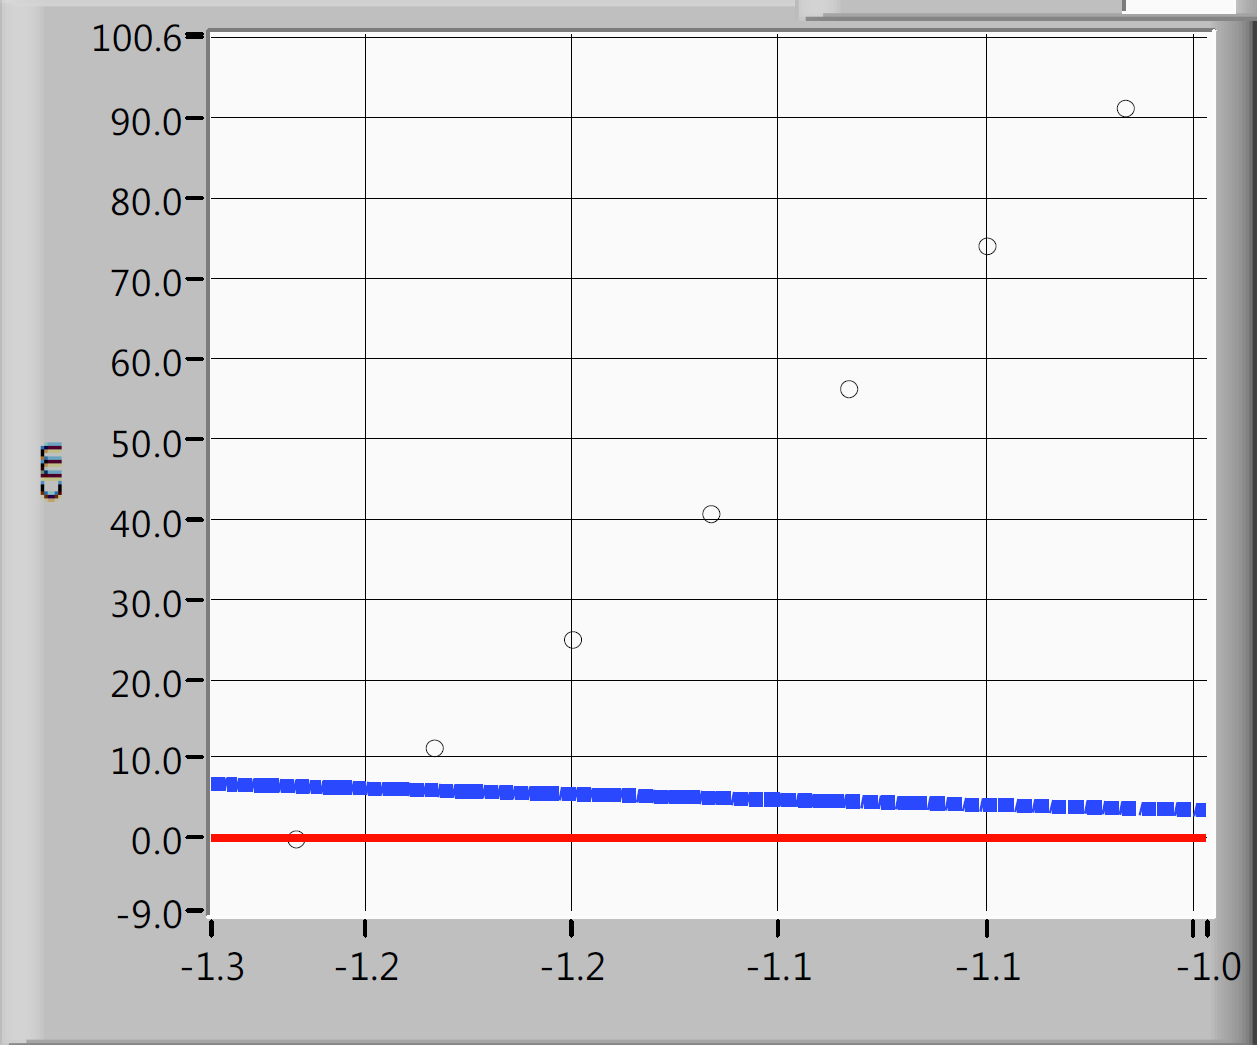
\includegraphics[scale=0.47]{r1p.png}
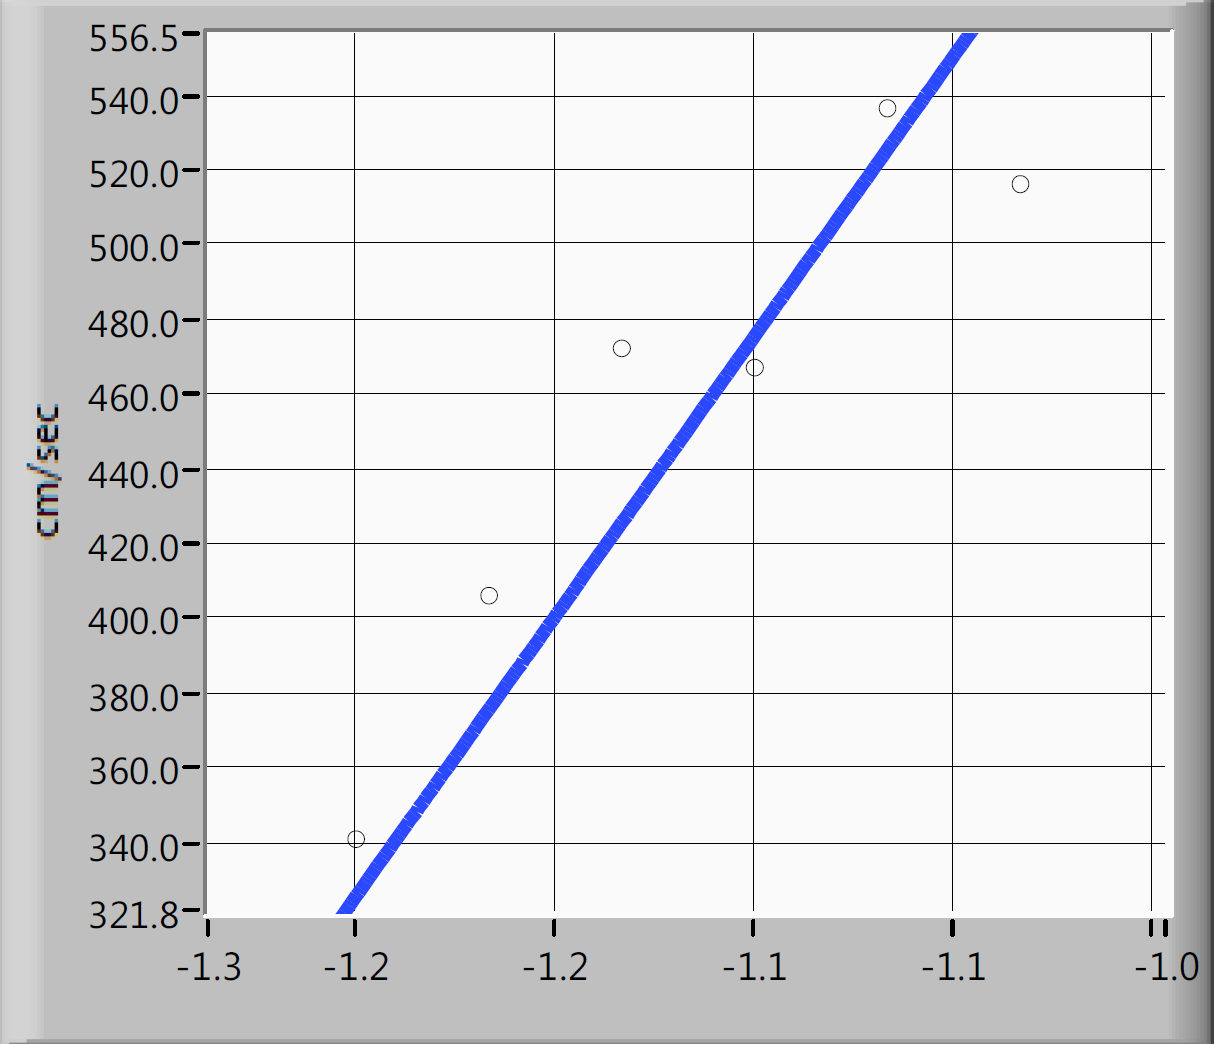
\includegraphics[scale=0.47]{r1v.png}
\textit{Left: Figure 1.} Motionlab Position v. Time graph \textit{Right: Figure 2.} Motionlab Velocity v. Time graph
\newline
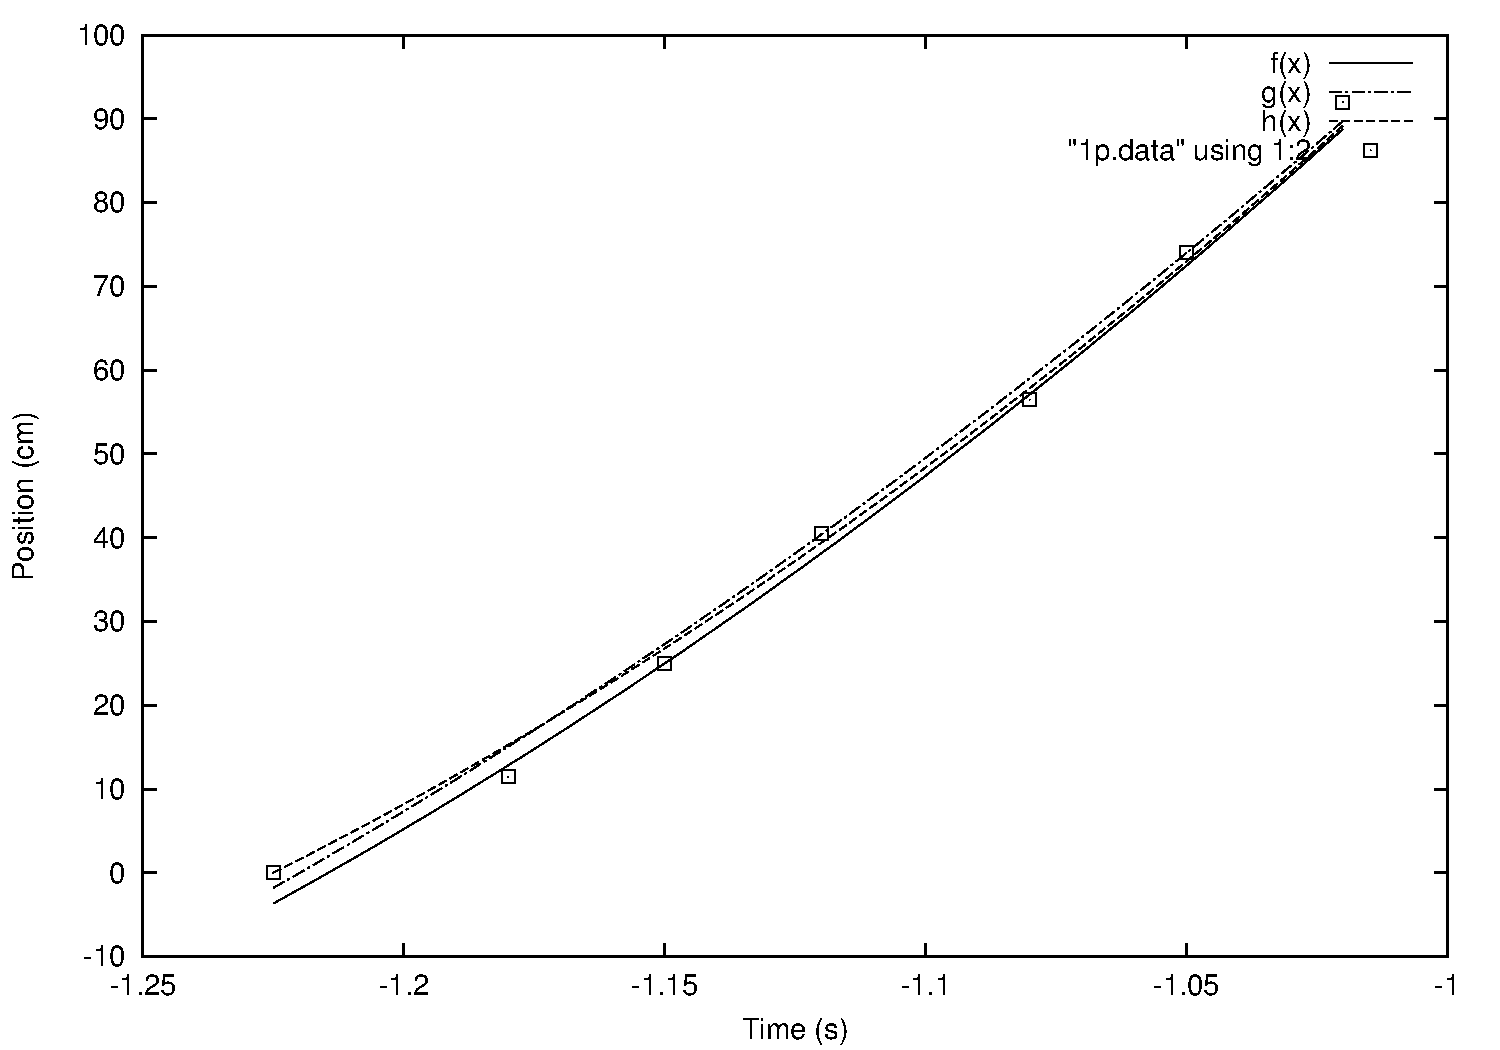
\includegraphics[scale=0.6]{1p.png}
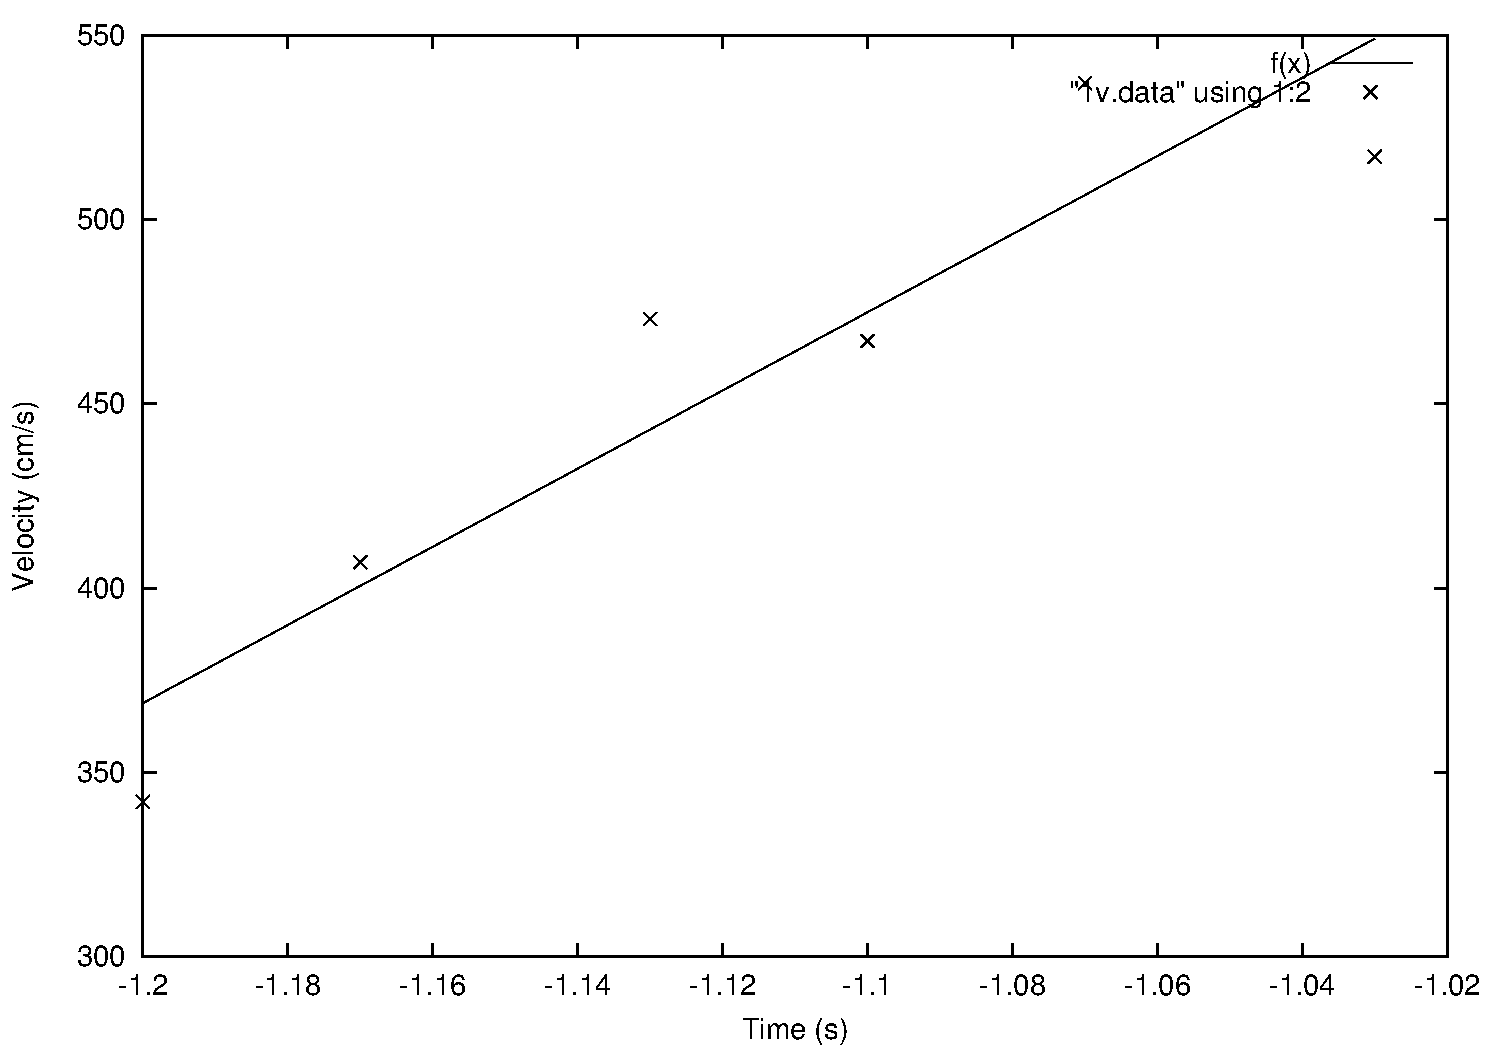
\includegraphics[scale=0.6]{1v.png}

\textit{Left: Figure 3.} Position v. time for trial 1

\(f(t) = 530t^2 + 1641t + 1212\), derived from line of best fit for \(v(t)\)

\(g(t) = 449t^2 + 1454t + 1106\), lower tolerance

\(h(t) = 600t^2 + 1782t + 1282.5\), upper tolerance

\textit{Right: Figure 4.} Velocity v. time for trial 1 

\(f(t) = 1060.5t + 1641\), best fit line using linear regression
\newline\newline
\textbf{Trial 2}
\newline\newline
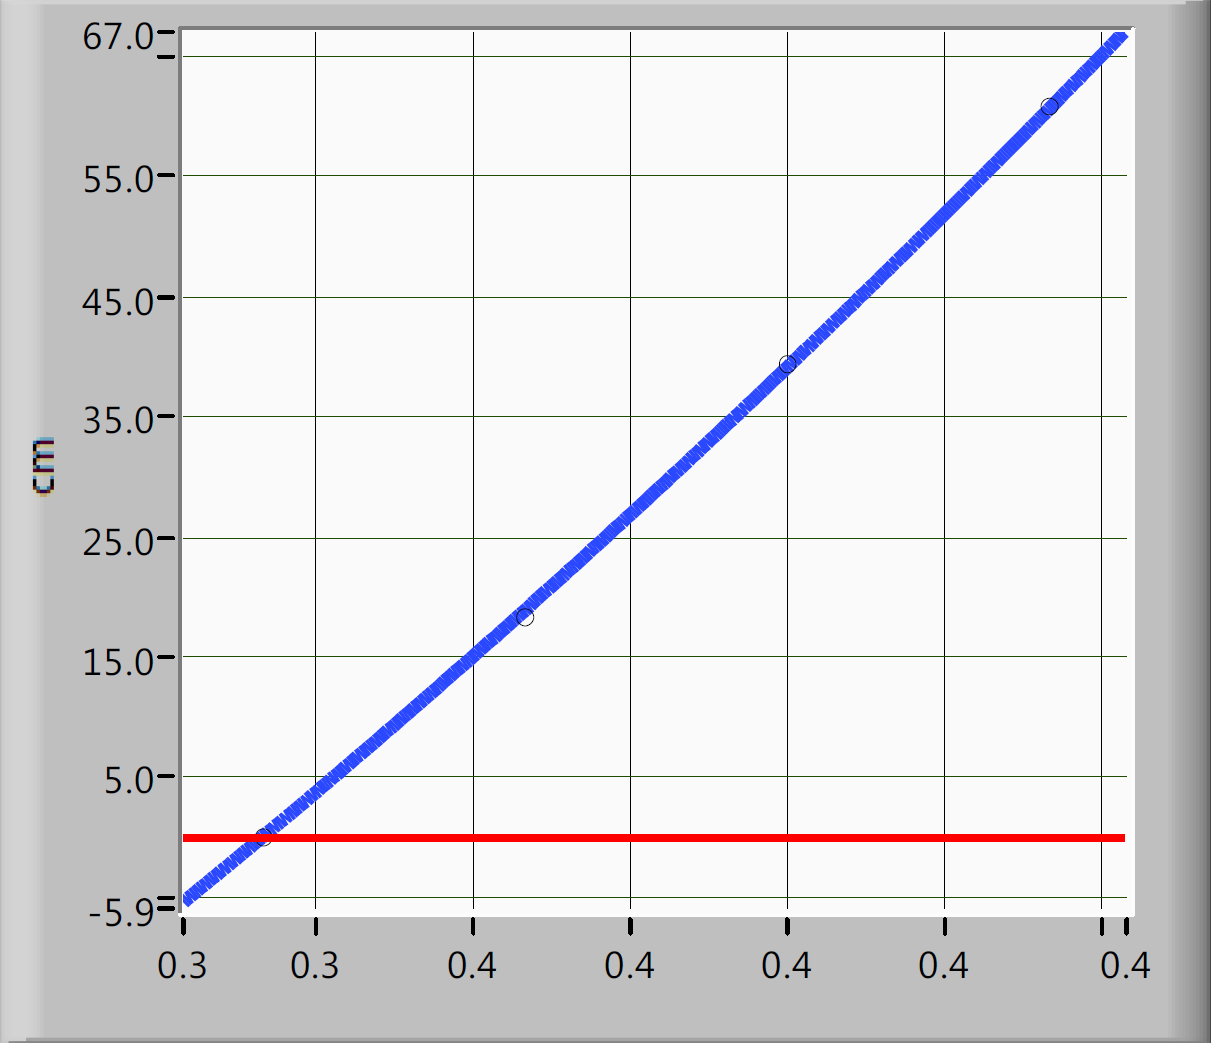
\includegraphics[scale=0.47]{r2p.png}
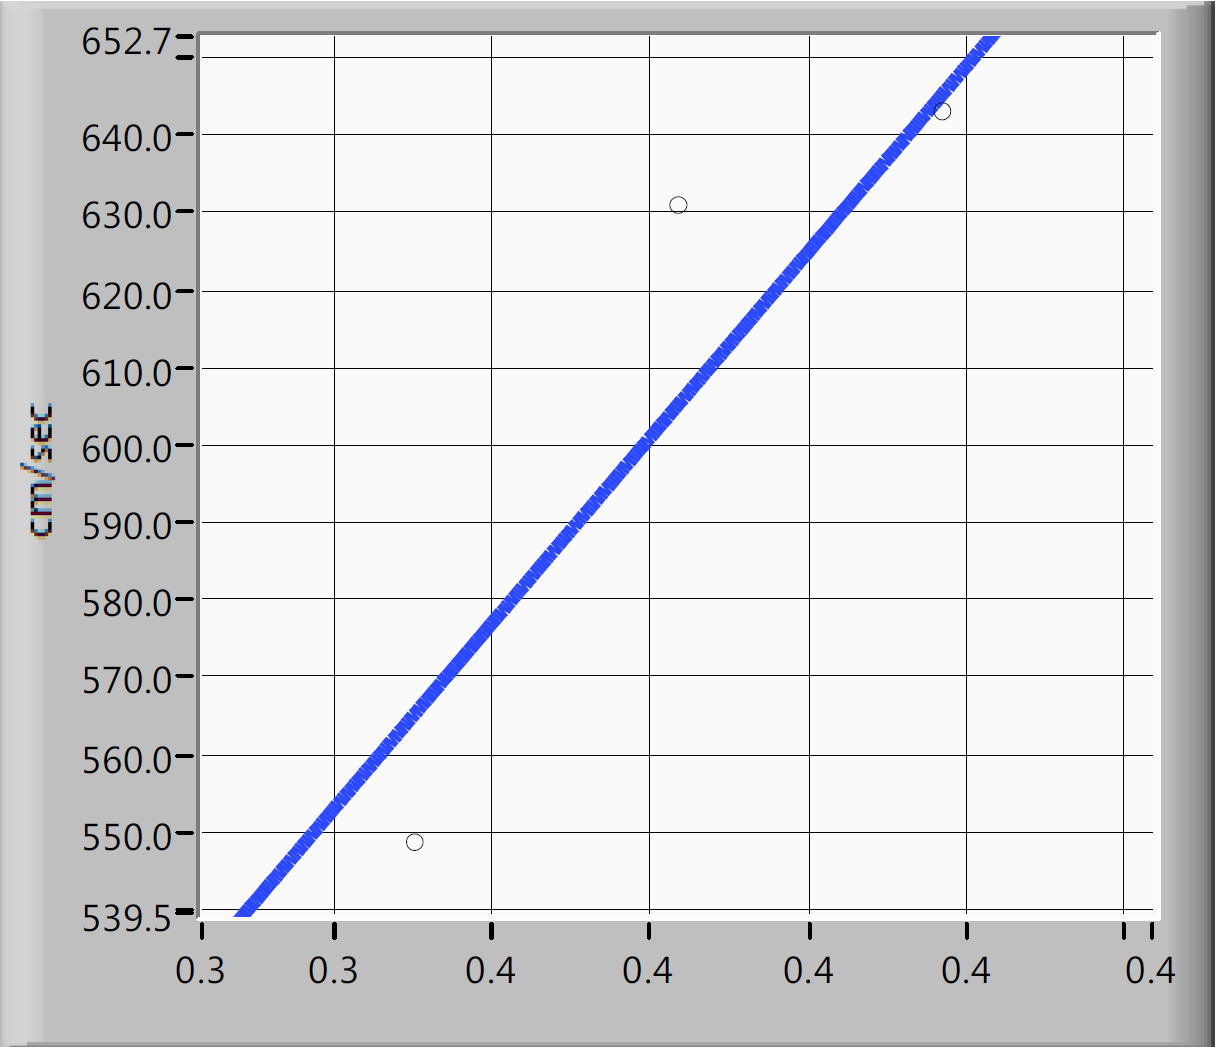
\includegraphics[scale=0.47]{r2v.png}
\newline
\textit{Left: Figure 5.} Motionlab Position v. Time graph \textit{Right: Figure 6.} Motionlab Velocity v. Time graph
\newline
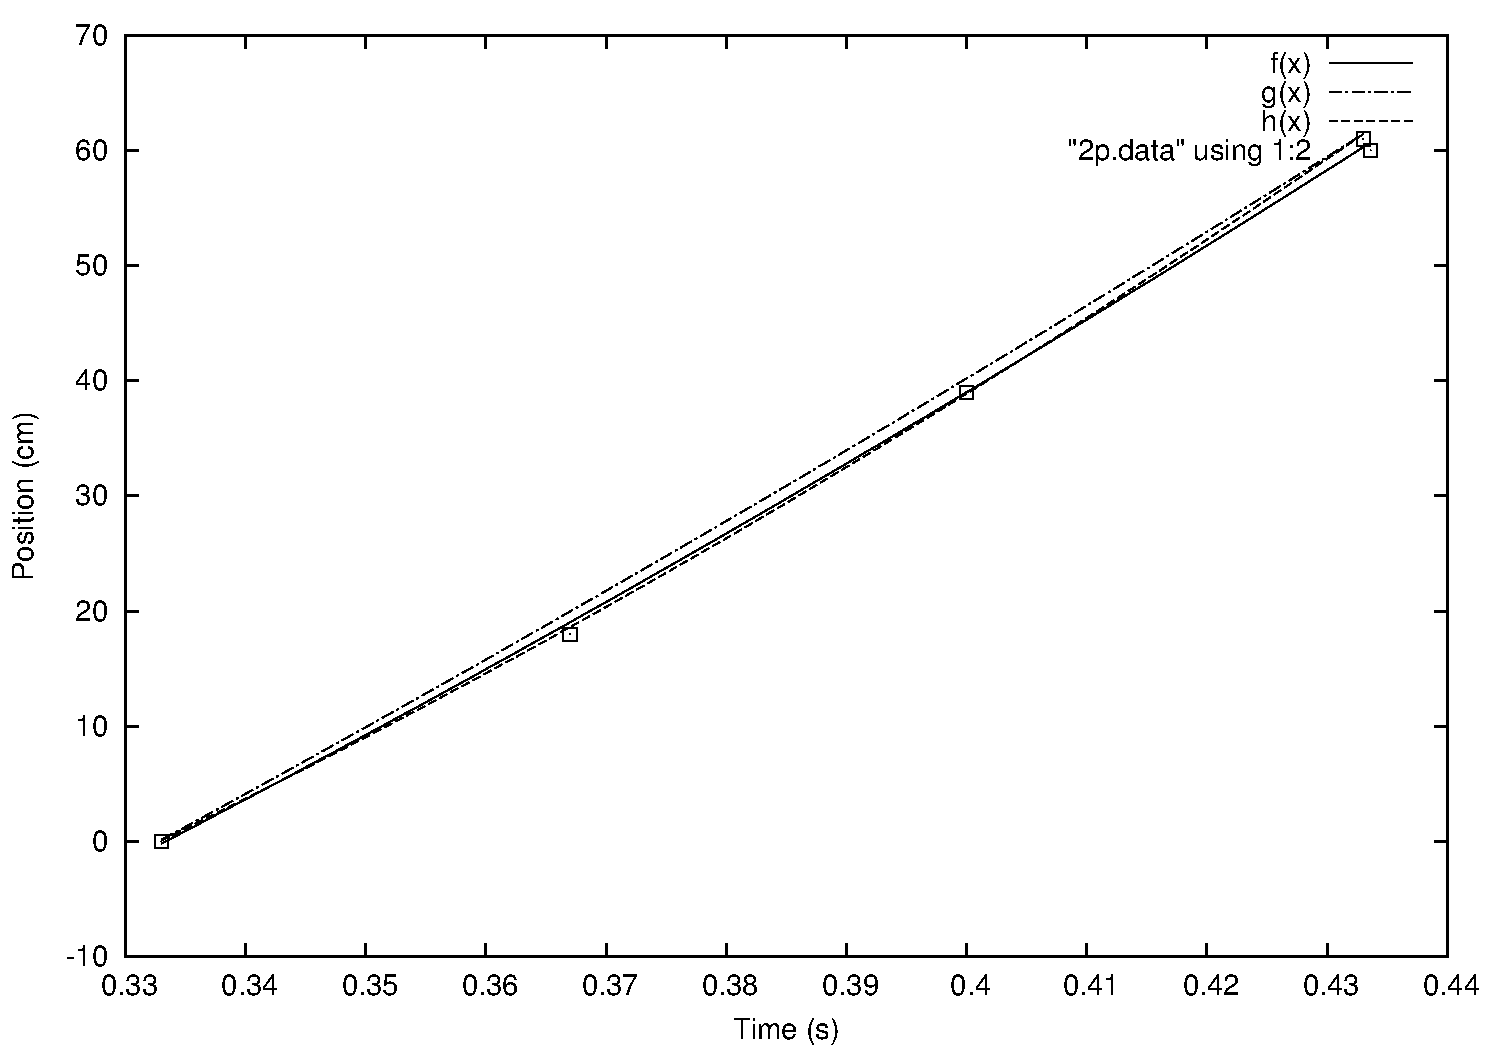
\includegraphics[scale=0.6]{2p.png}
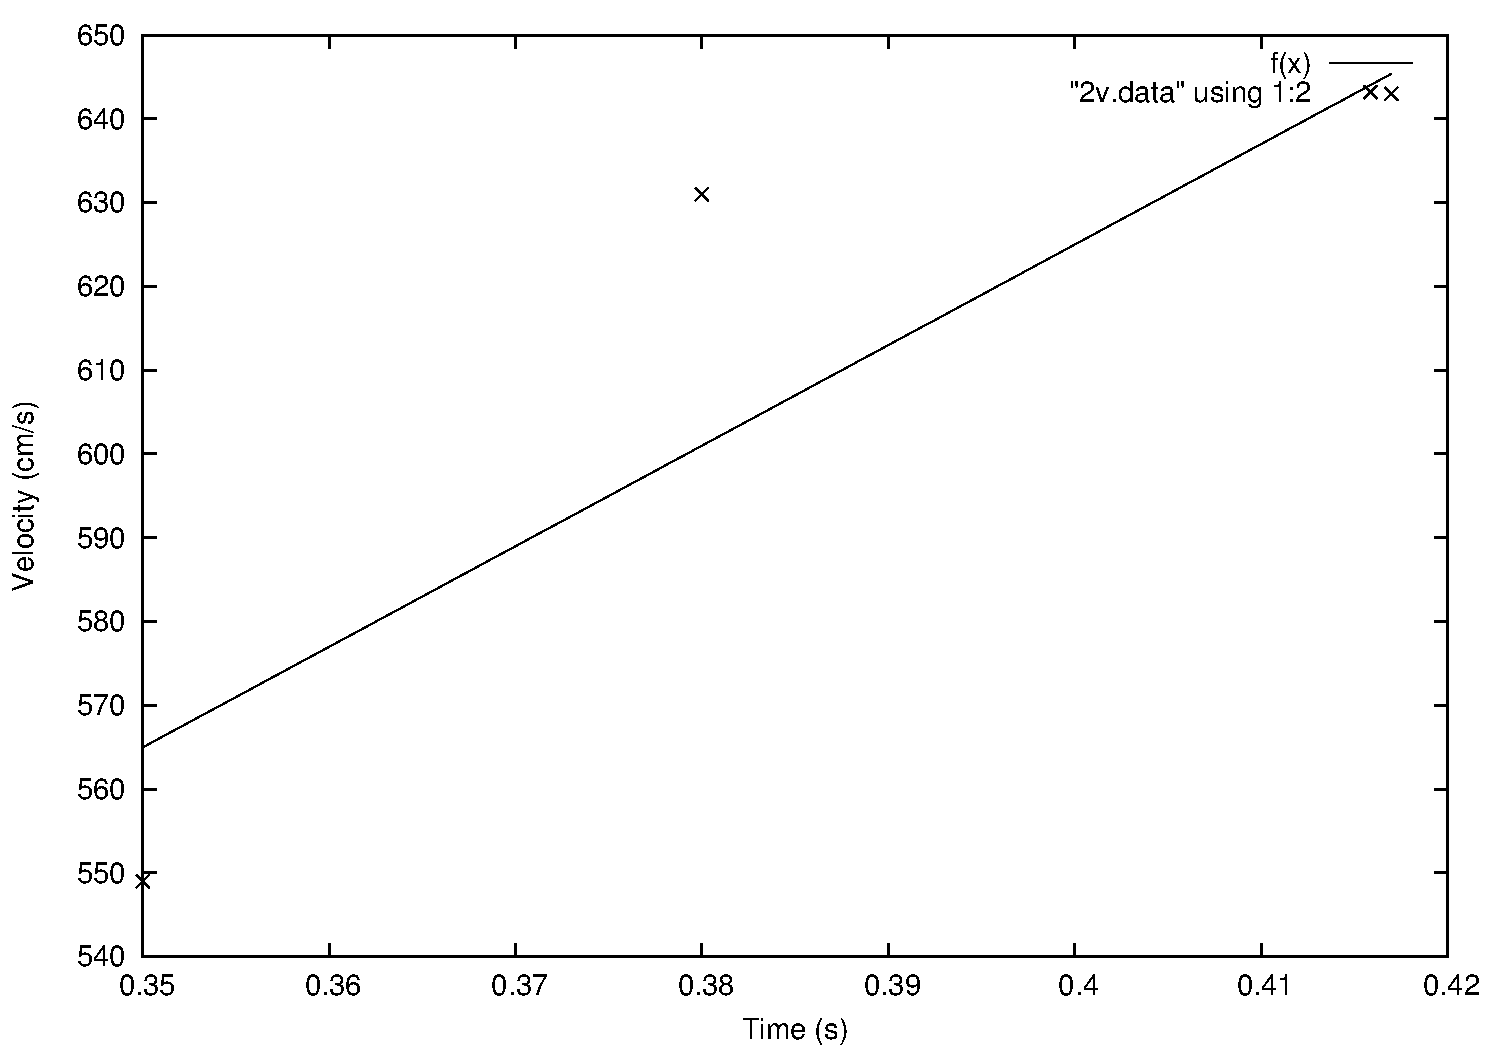
\includegraphics[scale=0.6]{2v.png}

\textit{Left: Figure 7.} Position v. time for trial 2

\(f(t) = 600t^2 + 145t - 115\), derived from \(v(t)\) line of best fit

\(g(t) = 450t^2 + 268t -139\), lower tolerance

\(h(t) = 1038t^2 - 182.5t -54.4\) , upper tolerance

\textit{Right: Figure 8.} Velocity v. time for trial 2

\(f(t) = 1200t + 145\), visually best fitted line
\newline\newline

\textbf{Trial 3}
\newline\newline
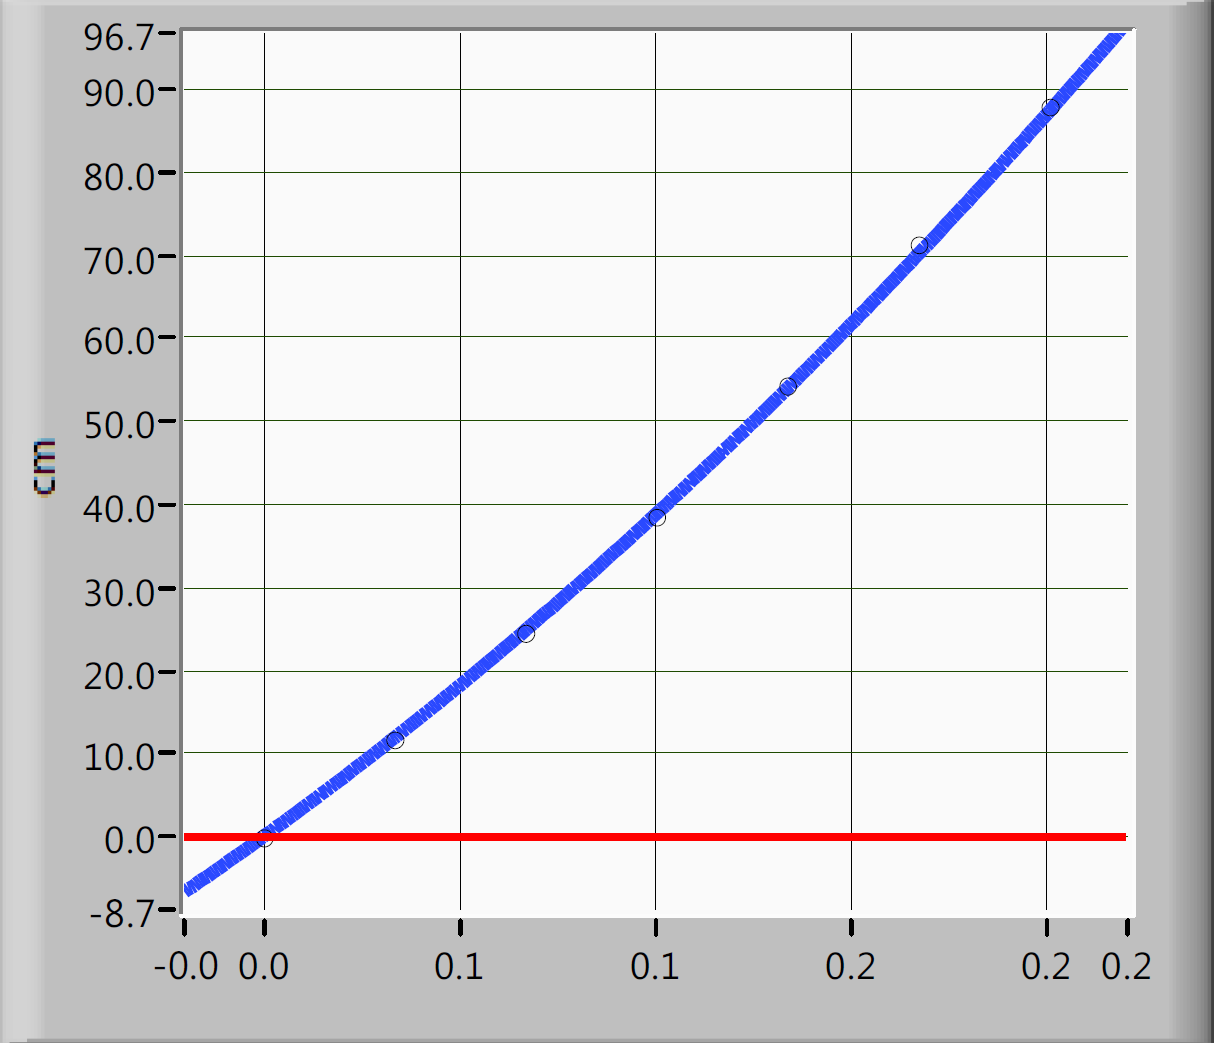
\includegraphics[scale=0.47]{r3p.png}
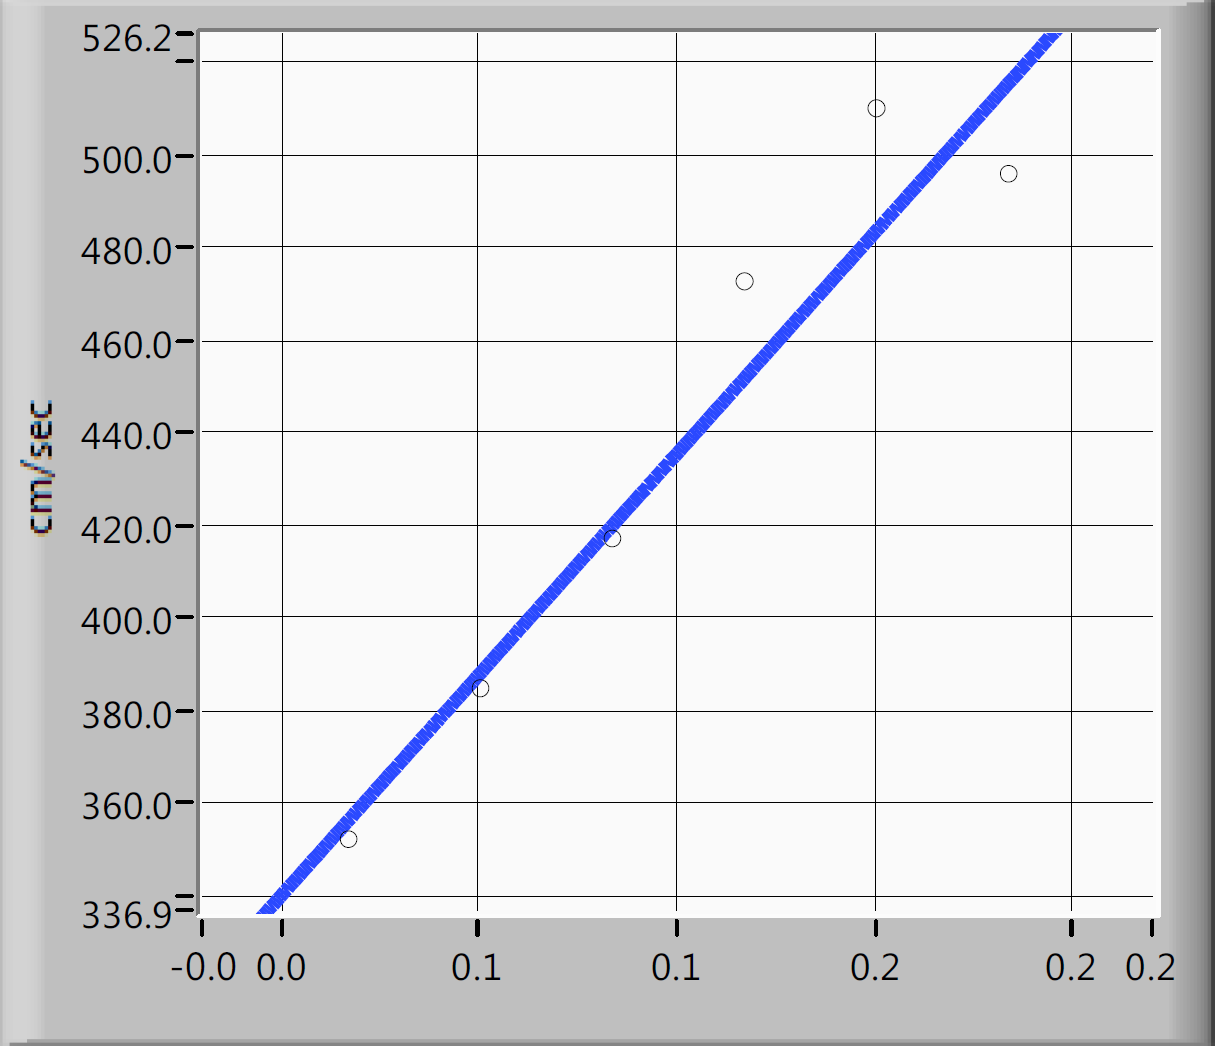
\includegraphics[scale=0.47]{r3v.png}
\textit{Left: Figure 9.} Motionlab Position v. Time graph \textit{Right: Figure 10.} Motionlab Velocity v. Time graph
\newline
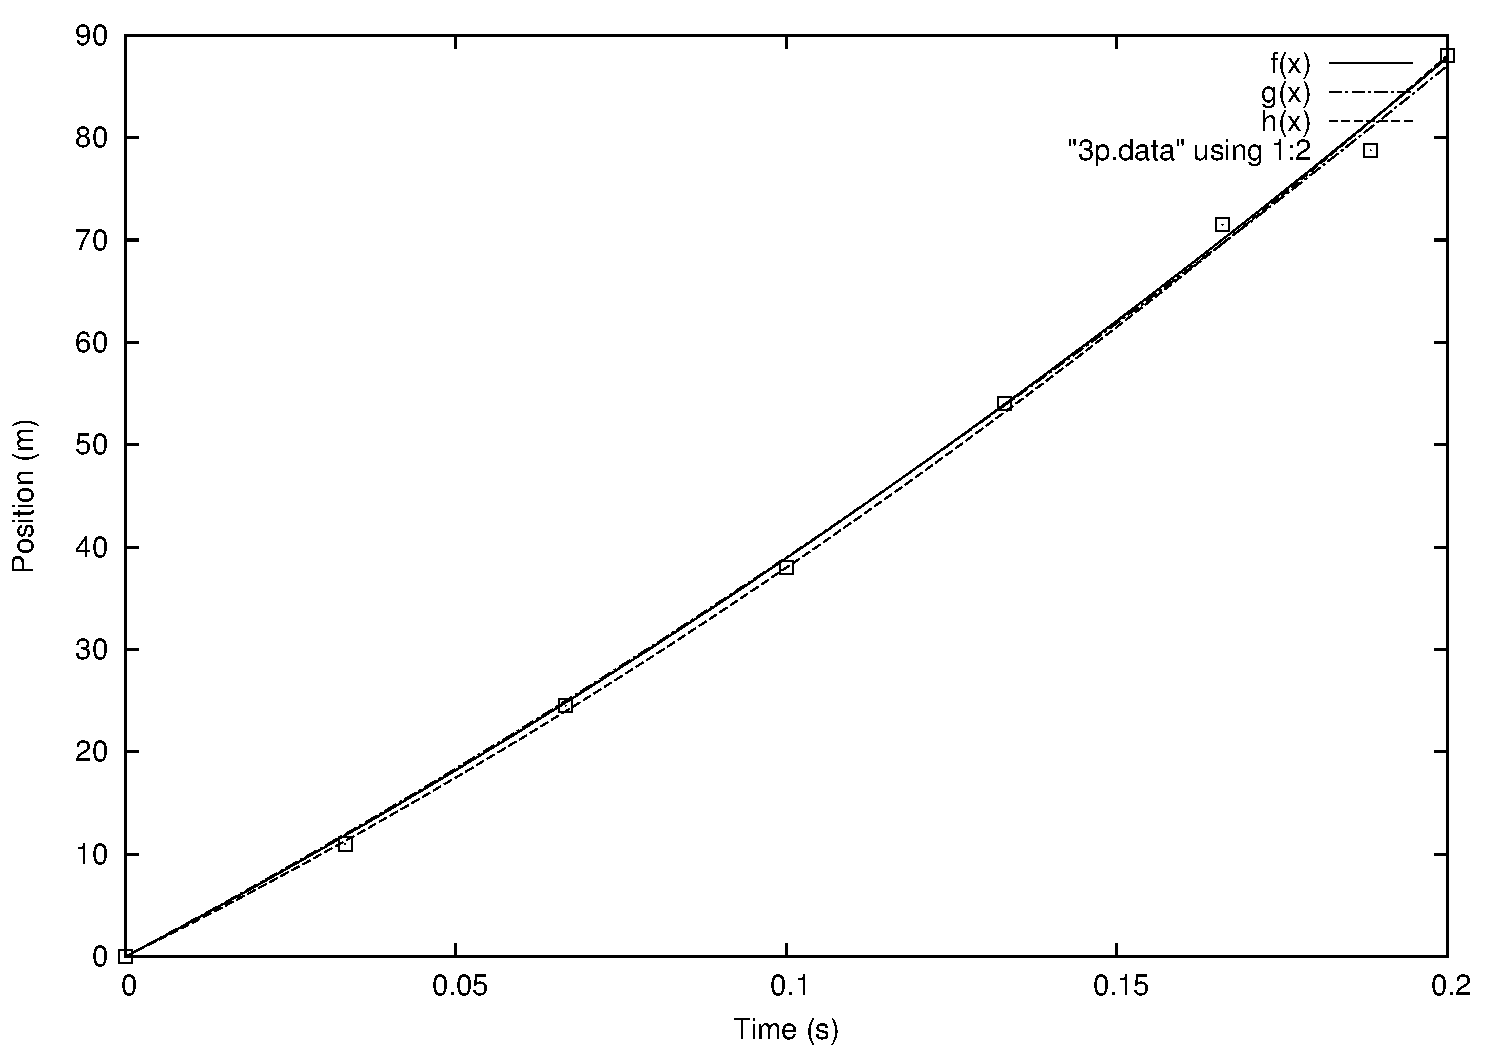
\includegraphics[scale=0.6]{3p.png}
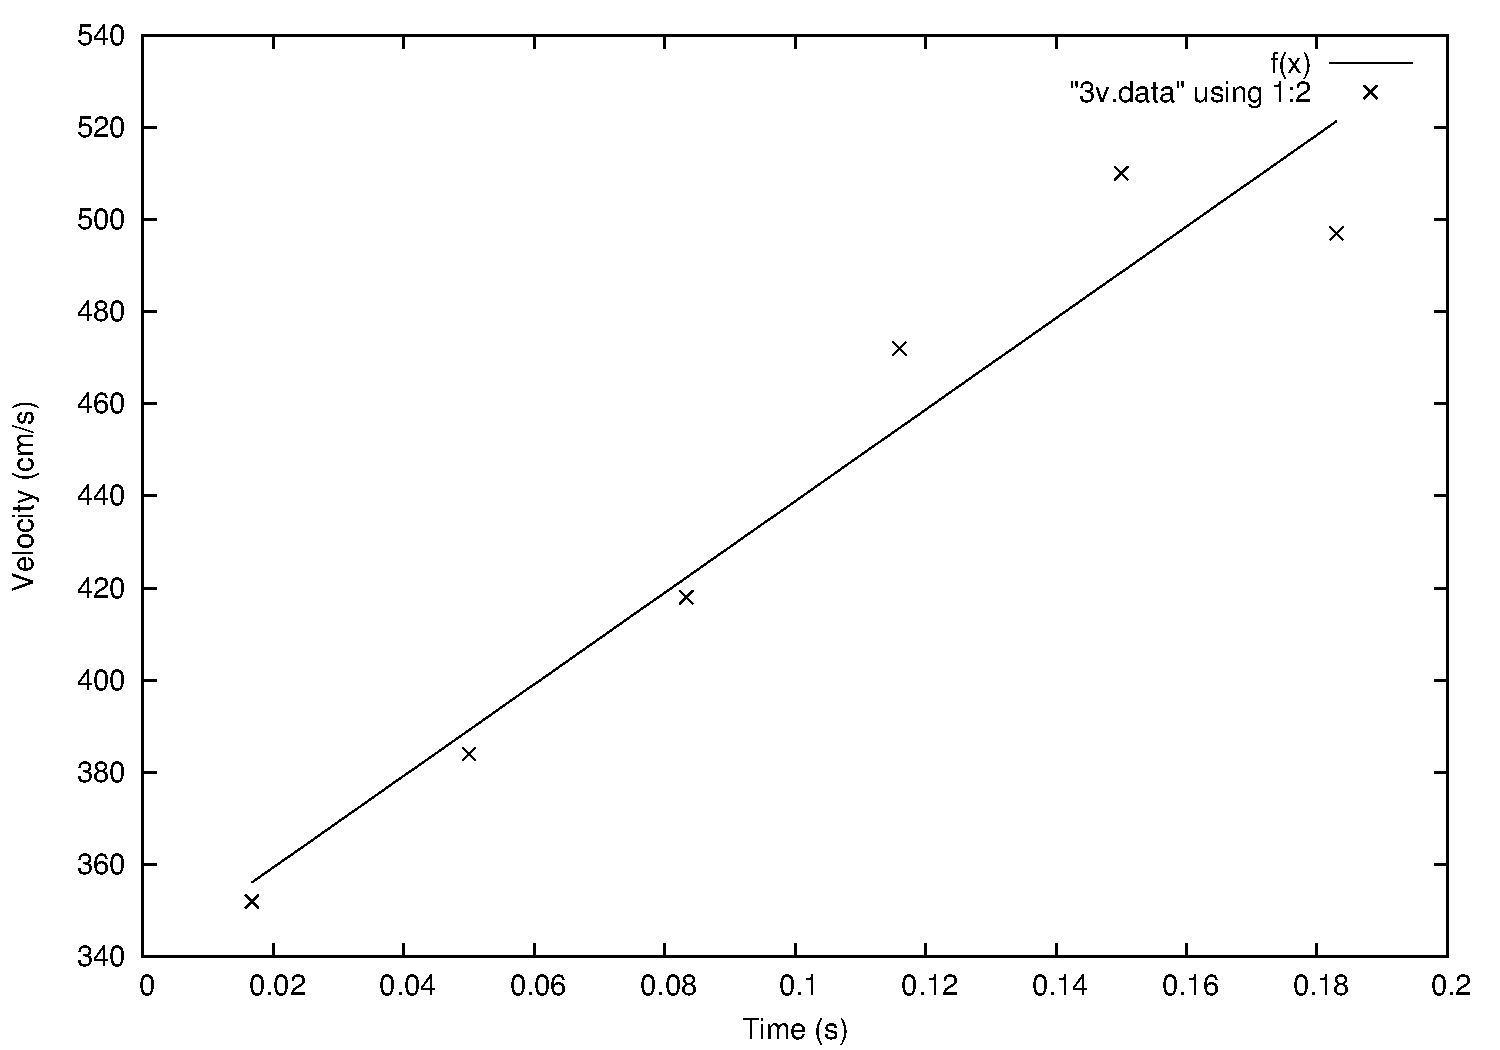
\includegraphics[scale=0.6]{3v.png}

\textit{Left: Figure 11.} Position v. time for trial 3 

\(f(t) = 497t^2 + 339.5t\), derived from \(v(t)\) line of best fit

\(g(t) = 450t^2 + 345t\), lower tolerance

\(h(t) = 600t^2 + 320t\) , upper tolerance

\textit{Right: Figure 12.} Velocity v. time for trial 3

\(f(t) = 993.5t + 339.5\), line of best fit found using linear regression
\newpage
\section{Analysis}
In order to show the independence of acceleration from initial velocity from the data gained in this experiment, several things will be done below. First, the initial velocity of each trial will be found to show that each trial started with a different initial velocity. Then the acceleration for each trial will be calculated and compared to see that the acceleration is constant across every trial. Finally it will be concluded that acceleration is independent of initial velocity because the acceleration in each trial was constant despite different initial velocities.
\newline\newline
\textbf{Velocity}
\newline
The initial velocity for each trial can be approximated using the velocity graph of each trial. It can be done by taking the value for the velocity of the line of best at the time of the first data point aquired by Motionlab . This data is shown below in table 1 for all the trials. This data is significant to show that each trial started with a different initial velocity to prove that initial velocity and acceleration have no correlation.
\newline\newline
\textit{Below: Table 1.} Initial velocity for each trial.
{\renewcommand{\arraystretch}{1.2}
\begin{table}[h]
\hspace*{1.6in}
\begin{tabular}{ll}
Trial  \hspace{.75in} & Approximate Initial Velocity\\
\hspace{.14in}1&\hspace{.7in}370 \(\frac{cm}{s}\)\\
\hspace{.14in}2&\hspace{.7in}565 \(\frac{cm}{s}\)\\
\hspace{.14in}3&\hspace{.7in}355 \(\frac{cm}{s}\)\\                 
\end{tabular}
\end{table}
\newline
}
\textbf{Acceleration}
\newline
Acceleration can be found simply by taking the second derivative of any position function of time. So, in order to find the acceleration of the ball in the trials, all one must do is calculate the second derivative of the position functions in the above data. The second derivative of the curve of best fit equation (\(f(t)\) for each trial) will be the approximate acceleration for each scenario, and the upper (\(g(t)\)) and lower tolerance (\(h(t)\)) functions will be the respective upper and lower tolerances for the acceleration. Mathematically (where function \(p(t)\) represents any of the position functions):
\begin{equation}
\frac{d^2p(t)}{dt^2} = \frac{dv(t)}{dt} = a(t) 
\end{equation}

\textit{Below: Table 2.} Lists the acceleration (\(\frac{d^2p(t)}{dt^2}\)) for each function \(f(t)\), \(g(t)\) and \(h(t)\) of each trial. The units of acceleration for the data under the \(\frac{d^2p(t)}{dt^2}\) columns is \(\frac{cm}{s^2}\).
{\renewcommand{\arraystretch}{1.2}
\begin{table}[h]
\hspace*{1.1in}
\begin{tabular}{ll|ll|ll}
Trial 1 \hspace{12pt} & \(\frac{d^2p(t)}{dt^2}\)\hspace{12pt} & \hspace{12pt}Trial 2 \hspace{12pt}& \(\frac{d^2p(t)}{dt^2}\)\hspace{12pt} & \hspace{12pt}Trial 3 \hspace{12pt}&\(\frac{d^2p(t)}{dt^2}\)\\
\(f(t)\)       & 1060     & \hspace{12pt}\(f(t)\)   & 1200   & \hspace{12pt}\(f(t)\)   &  994\\
\(g(t)\)       & 898      & \hspace{12pt}\(g(t)\)   & 900    & \hspace{12pt}\(g(t)\)   &  900\\
\(h(t)\)       & 1200     & \hspace{12pt}\(h(t)\)   & 2076   & \hspace{12pt}\(h(t)\)   &  1200\\                 
\end{tabular}
\end{table}
}
\newline
To determine the the acceleration of each trial with tolerances, it is simply equal to the value for acceleration found from the best fit curve \(f(t)\) plus (tolerance) the difference between the acceleration value for the \(h(t)\) and \(f(t)\) functions and minus (tolerance) the difference between the acceleration value from the \(f(t)\) and \(g(t)\) functions. In equation form:
\begin{equation}
acceleration =\frac{d^2f(t)}{dt^2} \hspace{3pt} \frac{+\frac{d^2h(t)}{dt^2} - \frac{d^2f(t)}{dt^2}}{-\frac{d^2f(t)}{dt^2} - \frac{d^2g(t)}{dt^2}}
\end{equation}
\textit{Below: Table 3.} Contains the found experimental acceleration for each trial with tolerances using equation 3.
{\renewcommand{\arraystretch}{1.2}
\begin{table}[h]
\hspace*{1.6in}
\begin{tabular}{ll}
Trial  \hspace{.75in} & Acceleration (with tolerance)\\
\hspace{.14in}1&\hspace{.4in}1060\hspace{2pt}\(\frac{+140}{-162}\) \(\frac{cm}{s^2}\)\\
\hspace{.14in}2&\hspace{.4in}1200\hspace{2pt}\(\frac{+876}{-300}\) \(\frac{cm}{s^2}\)\\
\hspace{.14in}3&\hspace{.42in}994\hspace{2pt}\(\frac{+206}{-94}\) \(\frac{cm}{s^2}\)\\                 
\end{tabular}
\end{table}
\newline
\textbf{Independence of Acceleration from Inital Velocity}
\newline
From the data in table 3, it is visible that the acceleration remained experimentally consistent as the found values for acceleration are close together and the ranges for each trial overlap considerably. Importantly, the tolerance range of each trial contains (as predicted) the value for acceleration due to gravity (\(g\)) near Earth's surface, which is \(981 \frac{cm}{s^2}\). This and the consistency of the data strongly implies that in each trial the ball was influenced as expected solely by constant acceleration near Earth's surface due to gravity. A constant acceleration over the three trials, despite having three different initial velocities (shown in table 1) suggests the validity of acceleration being independent of initial velocity.
\newline\newline
\textbf{Error}
\newline
There are several unaddressed sources of potential error in this experiment. The first source of potential error is due to barrel distortion in the camera that distorts the image on the edges of the frame. To limit this, one could avoid taking data from near the edges of the frame. We were unable to do so in all of our tests, namely in trial 2, so this has likely lead to some error. Another source of error is using the ball as the calibration object in Motionlab for trials 1 and 2. This would have yielded errors because a small object (the ball) gives the software a small amount of pixels in the image to calibrate off of, which magnifies the error. We rectified this in the third trial by using a meter stick as the calibration object. A third source of error is neglecting air resistance, which could have affected the acceleration as the velocity increased. These potential errors, however, do not seem to have yielded a very large amount of deviation in the results, as our data has  a fair level of consistency and reflect accurately on our predictions, which were the acceleration would be constant at \(g\) regardless of initial velocity.

\section{Conclusion}
Tennis balls were projected downwards with several different initial velocities. The independence of acceleration from initial velocity was confirmed.
\newline\newline
This result implies that there should be no concern over whether the the initial velocity of the air quality testing apparatus will affect the acceleration of the device in such a way that could damage it. This is because there is no correlation in the scenario (neglecting air resistance) between acceleration and the apparatus' initial velocity.


\end{document}